
\clearpage
\section {Implementation of Satisfiability Algorithm}
\subsection{Description}

The practical part of the project involved encoding all the above formalisms
and then writing in the translations.
The most difficult part was choosing the right encodings.

As an approximation to the problem I tried writing a Haskell program to decide satisfiability for LTL.

I wrote a haskell program to try to answer the satisfiability question for LTL.
I did this by translating LTL formulae into equivalent deterministic finite automata,
using basic automata and combinators, and testing for emptiness.
For example, I translated $\phi$ Until $\psi$ as:
\begin{code}
> ltl2aut (Until f1 f2) = (dStar $ ltl2aut f1) `dConc` ltl2aut f2
\end{code}

i.e. $ ltl2aut(\phi)^* \cdot ltl2aut(\psi) $.
But this was an error (I copied the translation of LTL to LDL in \cite{ldlf} which incorrectly translated $ f(\phi \, \mathcal{U} \, \psi) $ to $\langle f(\phi)^* \rangle f(\psi)$).
The correct translation of $ f(\phi \, \mathcal{U} \, \psi) $ into LDL is $\langle (f(\phi)?true)^* \rangle f(\psi)$. It doesn't seem simple to translate this directly to a DFA. So it makes sense to translate it (through LDL) to an AFA, as shown in \cite{ldlf}.

These were the issues that came up in coding:

The first was suitable representation of logics and automata.
In my first attempts the data types were not general enough
to cope with multiple logics and automata.
Particularly with doubly recursive types like LDLogic.
To solve this I made heavy use of Haskell's parameterised data types,
type synonyms and newtypes.
I decided it was not necessary to go all the way down to DFAs from
AFAs, and stopped at NFAs, since
emptiness of an AFA can be determined by looking at
the final state set of the corresponding NFA.

The second was the size of the automata.
The subset construction of an AFA produces an
NFA with exponentially many states.

As a partial solution, I only constructed reachable states.
But there will be cases for which reachability does not prune many states
(i.e. all states are reachable).
\red{not really sure what else I can do to make the whole satisfiability
procedure faster...}


I think there were some cases where Haskell got in the way, such as...
Hard to define "ShowSet" for arbitrarily nested sets.
Can't easily make predefined types into instances of stuff.
Need to do this newtype thing. Not extensible like Ruby.
Would have to edit original source code of predefined type.

Thus, all the pretty-printing is ad-hoc.

On the other hand, rigid though it can be,
it's nice to have that clean marking
of different types for different logics.
\red{a bit hand wavy}

\red{STUB}
Here is an example of my program...
the stages of data structures passed through on the way
to satisfiability.
do I need to construct this by hand?
I will show the output of my program for three different example formulae.

The first is actually a translation of an \ltlf formula
$(\lnext\lnext a) \luntil b$. Its translation is
$\di{(\di{true;true}a?;true)^*}b$.
Figures \ref{fig:until_printout_afa} and \ref{fig:until_printout_nfa}
show the output of the program
I have written, which translates the \ldlf formula into an AFA and thence into an NFA.
Satisfiability can be determined by looking at the final state set of the NFA, since
the program constructs only the reachable states of the automaton.
If the final state set is nonempty, then the formula is satisfiable.
Figure \ref{fig:until_afa} is a diagram of the AFA detailed in \ref{fig:until_printout_afa}.
Figure \ref{fig:until_afa_simp} simplifies the $\lor$s out of the automaton
by rules of logical equivalence.
Looking at figure \ref{fig:until_afa_simp} we can see that
the trace $\set{}\set{}\set{b}$ would cause the automaton
to fail. After consuming $\set{}$, $\set{}\set{b}$ must be accepted from $q_2$,
since we go via a $\land$ node. But $\set{}\set{b}$ leads the automaton exactly
into the $False$ transition. Thus the whole run fails. Indeed, we can see that
$\set{}\set{}\set{b} \not\models \lnext\lnext a$ and also $\not\models b$, so this is to be expected.

\usetikzlibrary{shapes,shapes.geometric,arrows,fit,calc,positioning,automata,}
\tikzset{rectangular state/.style={draw,rectangle,minimum width=1cm,minimum height=1cm}}

\begin{figure}
\begin{printout}
====================================================================================================
LDL: <(<(True;True)>a?;True)*>b
------------------------------------------------------------
AFA: Alphabet: {{}, {a}, {a, b}, {b}}
States: {a, <True>a, <(<(True;True)>a?;True)*>b}
Init: <(<(True;True)>a?;True)*>b
Transition: a X {} -> False
a X {a} -> True
a X {a, b} -> True
a X {b} -> False
<True>a X {} -> state(a)
<True>a X {a} -> state(a)
<True>a X {a, b} -> state(a)
<True>a X {b} -> state(a)
<(<(True;True)>a?;True)*>b X {}
  -> (False || (state(<True>a) && state(<(<(True;True)>a?;True)*>b)))
<(<(True;True)>a?;True)*>b X {a}
  -> (False || (state(<True>a) && state(<(<(True;True)>a?;True)*>b)))
<(<(True;True)>a?;True)*>b X {a, b}
  -> (True || (state(<True>a) && state(<(<(True;True)>a?;True)*>b)))
<(<(True;True)>a?;True)*>b X {b}
  -> (True || (state(<True>a) && state(<(<(True;True)>a?;True)*>b)))

Final: {}
\end{printout}
\caption{Printout of ``Until'' formula results (AFA) \label{fig:until_printout_afa}}
\end{figure}
\begin{figure}
  \begin{printout}
------------------------------------------------------------
NFA: Alphabet: {{}, {a}, {a, b}, {b}}
States: {{}, {a}, {a, <True>a, <(<(True;True)>a?;True)*>b},
{<True>a, <(<(True;True)>a?;True)*>b}, {<(<(True;True)>a?;True)*>b}}
Init: {<(<(True;True)>a?;True)*>b}
Transition: {} X {} -> {{}}
{} X {a} -> {{}}
{} X {a, b} -> {{}}
{} X {b} -> {{}}
{a} X {} -> {}
{a} X {a} -> {{}}
{a} X {a, b} -> {{}}
{a} X {b} -> {}
{a, <True>a, <(<(True;True)>a?;True)*>b} X {} -> {}
{a, <True>a, <(<(True;True)>a?;True)*>b} X {a} -> {{a, <True>a, <(<(True;True)>a?;True)*>b}}
{a, <True>a, <(<(True;True)>a?;True)*>b} X {a, b} -> {{a}}
{a, <True>a, <(<(True;True)>a?;True)*>b} X {b} -> {}
{<True>a, <(<(True;True)>a?;True)*>b} X {} -> {{a, <True>a, <(<(True;True)>a?;True)*>b}}
{<True>a, <(<(True;True)>a?;True)*>b} X {a} -> {{a, <True>a, <(<(True;True)>a?;True)*>b}}
{<True>a, <(<(True;True)>a?;True)*>b} X {a, b} -> {{a}}
{<True>a, <(<(True;True)>a?;True)*>b} X {b} -> {{a}}
{<(<(True;True)>a?;True)*>b} X {} -> {{<True>a, <(<(True;True)>a?;True)*>b}}
{<(<(True;True)>a?;True)*>b} X {a} -> {{<True>a, <(<(True;True)>a?;True)*>b}}
{<(<(True;True)>a?;True)*>b} X {a, b} -> {{}}
{<(<(True;True)>a?;True)*>b} X {b} -> {{}}

Final: {{}}

------------------------------------------------------------
Satisfiable? According to NFA's final state set, yes
====================================================================================================
\end{printout}
\caption{Printout of ``Until'' formula results (NFA) \label{fig:until_printout_nfa}}
\end{figure}

{
\newcommand{\rhoY}{\di{true;true}a?}
\newcommand{\rhoX}{\di{true;true}a?;true}
\begin{figure}
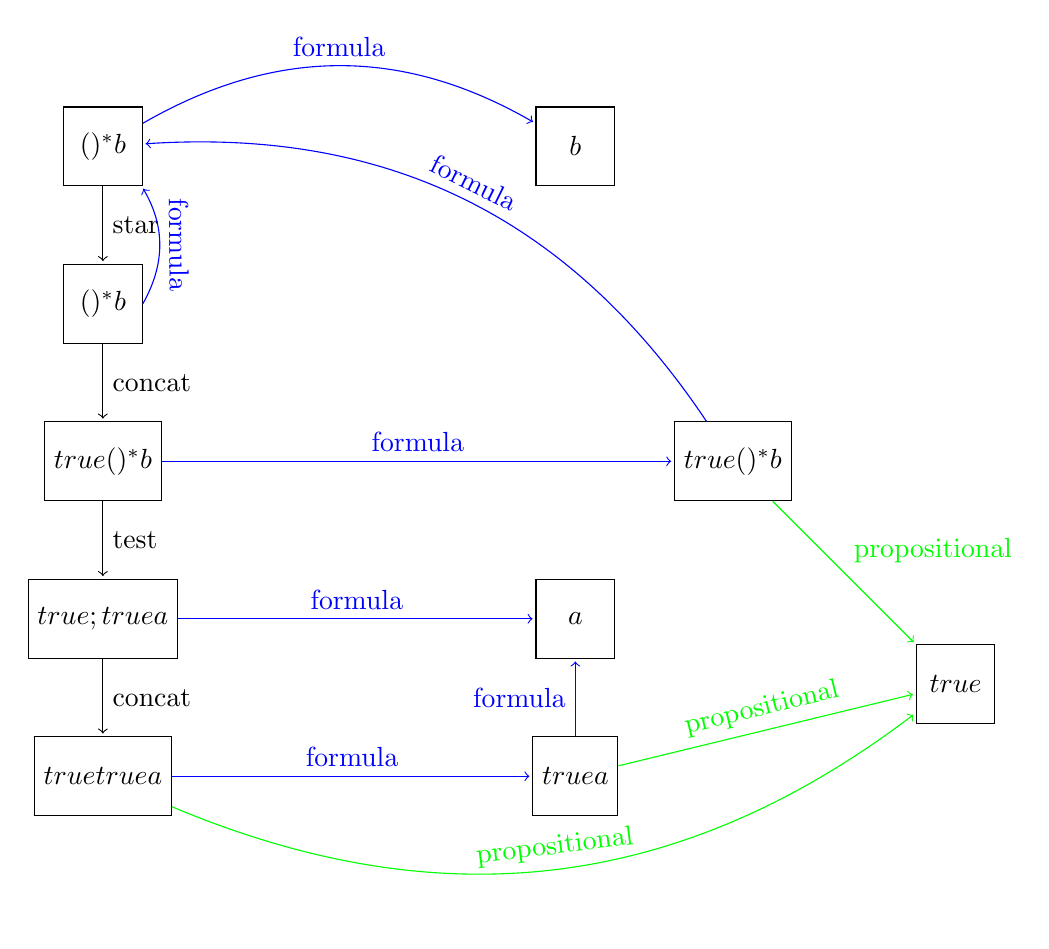
\begin{tikzpicture}[shorten >=1pt,node distance=2cm,on grid,auto]
  \node[rectangular state] (RXSTARB) {$\di{(\rhoX)^*}b$};
  \node[rectangular state] (B) [right of = RXSTARB, node distance = 6 cm] {$b$};
  \node[rectangular state] (RXRXSTARB) [below of = RXSTARB] {$\di{\rhoX}\di{(\rhoX)^*}b$};
  \node[rectangular state] (RYTRXSTARB) [below of = RXRXSTARB] {$\di{\rhoY}\di{true}\di{(\rhoX)^*}b$};
  \node[rectangular state] (TRXSTARB) [right of = RYTRXSTARB, node distance = 8 cm ] {$\di{true}\di{(\rhoX)^*}b$};
  \node[rectangular state] (T) [below right of = TRXSTARB, node distance = 4 cm] {$true$};
  \node[rectangular state] (TTA) [below of = RYTRXSTARB] {$\di{true;true}a$};
  \node[rectangular state] (A) [right of = TTA, node distance = 6 cm] {$a$};
  \node[rectangular state] (TTA2) [below of = TTA] {$\di{true}\di{true}a$};
  \node[rectangular state] (TA) [right of = TTA2, node distance = 6 cm] {$\di{true}a$};
  \path[->]
  (RXSTARB) edge [blue, bend left] node [sloped, above] {formula} (B)
            edge node {star} (RXRXSTARB)
  (RXRXSTARB.0) edge [blue, bend right] node [sloped, above] {formula} (RXSTARB)
  (RXRXSTARB)   edge node {concat} (RYTRXSTARB)
  (RYTRXSTARB) edge [blue] node {formula} (TRXSTARB)
                edge node {test} (TTA)
  (TRXSTARB) edge [blue, bend right] node [sloped, above] {formula} (RXSTARB)
              edge [green] node {propositional} (T)
  (TTA) edge [blue] node {formula} (A)
        edge node {concat} (TTA2)
  (TTA2) edge [blue] node {formula} (TA)
      edge [green, bend right] node [sloped, above] {propositional} (T)
  (TA) edge [blue] node {formula} (A)
      edge [green] node [sloped, above] {propositional} (T);
\end{tikzpicture}
\caption{Fisher-Ladner closure of formula $\di{(\di{true;true}a?;true)^*}b$
(not the showing negated formulae-- of which there are exactly one for each shown)} \label{fig:until_fl}
\end{figure}
}
\begin{figure}
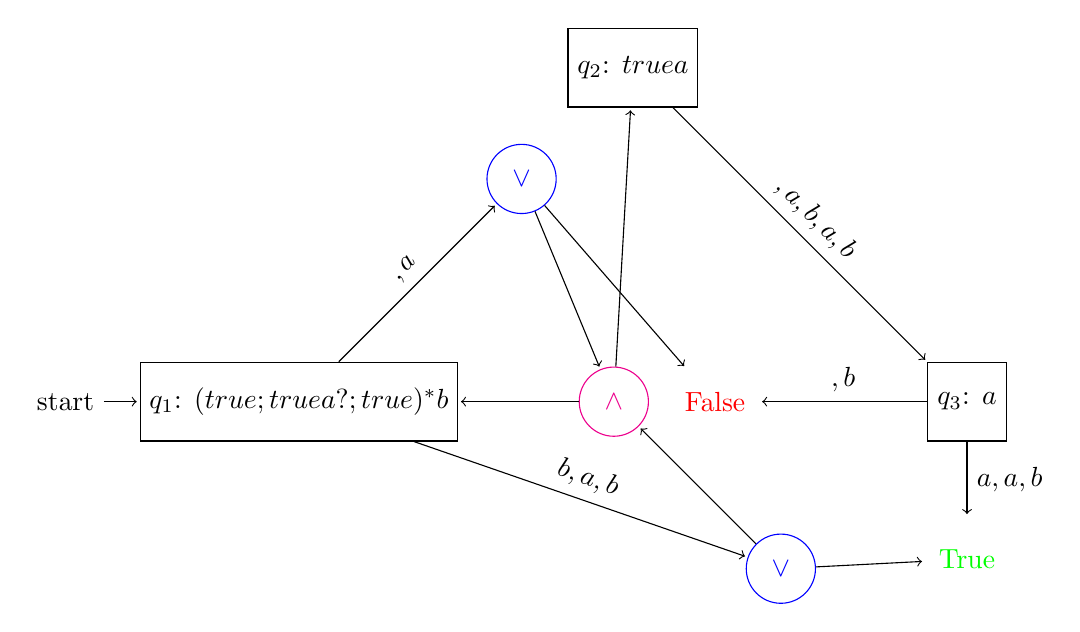
\begin{tikzpicture}[shorten >=1pt,node distance=2cm,on grid,auto]
   \node[initial, rectangular state] (q1)   {$q_1$: $\di{(\di{true;true}a?;true)^*}b$};
   \node[rectangular state] (q2) [above right of= q1, node distance = 6 cm] {$q_2$: $\di{true}a$};
   \node[rectangular state] (q3) [below right of= q2, node distance = 6 cm] {$q_3$: $a$};
   \node[state, draw=none, green] (true) [below of=q3] {True};
   \node[state, draw=none, red] (false) [left of = q3, node distance = 3.2 cm] {False};
   \node[state, magenta] (and) [right of = q1, node distance = 4 cm] {$\land$};
   \node[state, blue] (orFalse) [above right of = q1, node distance = 4 cm] {$\lor$};
   \node[state, blue] (orTrue) [below right of = and, node distance = 3 cm] {$\lor$};


    \path[->]
    (q3) edge node [sloped, above] {$\set{}, \set{b}$} (false)
         edge node {$\set{a}, \set{a,b}$} (true)
    (q2) edge node [sloped, above] {$\set{}, \set{a}, \set{b}, \set{a,b}$} (q3)
    (q1) edge node [sloped, above] {$\set{}, \set{a}$} (orFalse)
         edge node [align=center, sloped, above] {$\set{b}, \set{a,b}$} (orTrue)
    (and) edge node {} (q1)
          edge node {} (q2)
    (orFalse) edge node {} (and)
              edge node {} (false)
    (orTrue)  edge node {} (and)
              edge node {} (true);
\end{tikzpicture}
\caption{AFA constructed from formula (note that the states are a subset of the Fisher-Ladner closure)}\label{fig:until_afa}
\end{figure}


\begin{figure}
\begin{tikzpicture}[shorten >=1pt,node distance=2cm,on grid,auto]
   \node[initial, rectangular state] (q1)   {$q_1$: $\di{(\di{true;true}a?;true)^*}b$};
   \node[state, magenta] (and) [above right of = q1, node distance = 5 cm] {$\land$};
   \node[rectangular state] (q2) [right of= and, node distance = 4 cm] {$q_2$: $\di{true}a$};
   \node[rectangular state] (q3) [below of= q2, node distance = 4 cm] {$q_3$: $a$};
   \node[state, draw=none, green] (true) [below left of=q3, node distance = 4 cm] {True};
   \node[state, draw=none, red] (false) [left of = q3, node distance = 3.2 cm] {False};


    \path[->]
    (q3) edge node [sloped, above] {$\set{}, \set{b}$} (false)
         edge node [sloped, above] {$\set{a}, \set{a,b}$} (true)
    (q2) edge node {$\set{}, \set{a}, \set{b}, \set{a,b}$} (q3)
    (q1) edge [bend right] node [sloped, above] {$\set{}, \set{a}$} (and.315)
         edge node [sloped, above] {$\set{b}, \set{a,b}$} (true)
    (and) edge [bend right] node [align=center] {} (q1)
    (and)      edge node {} (q2);
\end{tikzpicture}
\caption{Simplified version of figure \ref{fig:until_afa}}\label{fig:until_afa_simp}
\end{figure}


\subsection{Evaluation and Comparison to existing tools}


\red{To do...}
Systems for managing automata, logic and games have been in development for quite some time, notably GOAL (and ...?).

I tried GOAL and here's how it compares with my system...

I would not expect my implementation to be as refined as such systems.

\subsection{Code listings}

First attempt


data structures


Second attempt


data structures
